\documentclass{article}
  \usepackage{amsmath}
  \usepackage{amssymb}
  \usepackage{graphicx}
  \usepackage{float}
\topmargin=-1.2cm \oddsidemargin=0.1cm \evensidemargin=0.1cm
\textwidth=16 true cm \textheight=23 true cm

\font\euler=EUSM10 \font\eulers=EUSM7

\begin{document}
\title{ECON 3610B International Trade \\Assignment $1^{\text{st}}$}
\author{{\normalsize Leonard Sheng(SHENG,Hao), 1155035947, via \LaTeX}}
\date{\today}

\maketitle
\baselineskip 0.6cm

\begin{description}
    \item[I.]{\bf Answer:}\\
        (2)4667 billion dollars; 26.20\%.\\
        (3)862 billion dollars; 31.04\%.\\
        (4)1686 billion dollars; 9.46\%.\\
        (5)9645 billion dollars; 54.13\%.\\
        (6)2039 billion dollars; 11.45\%.\\
        (7)34.42\%. It is the sum of CELL $[J40]$ and $[J42]$ in the original form.\\
        (8)When measured in billion dollars, generally, all the trade amount above are getting larger than the statistics of 2006(lecture slide 1-12). However, if we focus on the share of the world trade, things can be different. Trade within Europe, between Europe and North America, within Americas seems to lose their share of the total. And exports from Europe and Americas declines a little bit. On the other hand, exports(measured as the proportion of world total) from Asia, Middle East and CIS are increasing. Even Africa gets a 0.3\% increase.


    \item[II.]{\bf Answer:}\\
        (1)(a)The PPF is $2Q_B+3Q_A\leq 1200$,
            where $Q_B$ is the quantity of banana produced domestically, $Q_A$ is the quantity of apple produced at Home.\\
            \begin{center}
               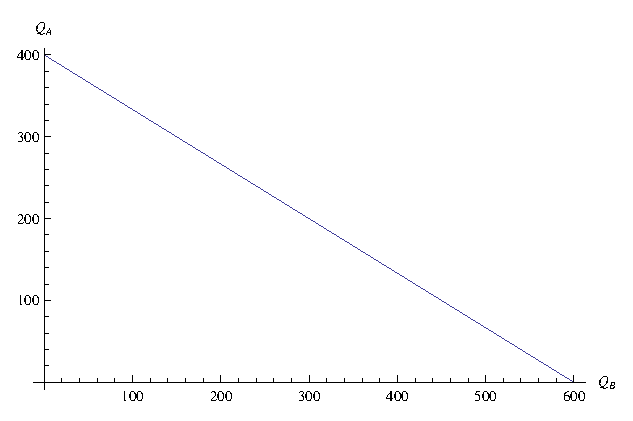
\includegraphics[angle=0, width=0.6\textwidth]{ECON3610A11}
            \end{center}
           (b)$\frac{3}{2}$ unit bananas.
           \\The labor required to produce one unit apple is 3 unit, which can otherwise be used to produce $\frac{3}{2}$ unit bananas\\
           (c)$\frac{P_A}{P_B}=\frac{3}{2}$.\\
           If the labor(people) can transfer from one sector to the other, the wages will be eventually be the same: $w^*=\frac{P_A}{a_A}=\frac{P_B}{a_B}$($w^*$ denotes the equilibrium wage). In this particular case, $\frac{P_A}{3}=\frac{P_B}{2}$, which makes the relative price of apple over banana $\frac{3}{2}$.  \\
        (2)(a)The PPF is $5Q^*{}_B+1Q^*{}_A\leq 800$,
            where $Q^*{}_B$ is the quantity of banana produced in Foreign, $Q^*{}_A$ is the quantity of apple produced oversea.\\
            \begin{center}
                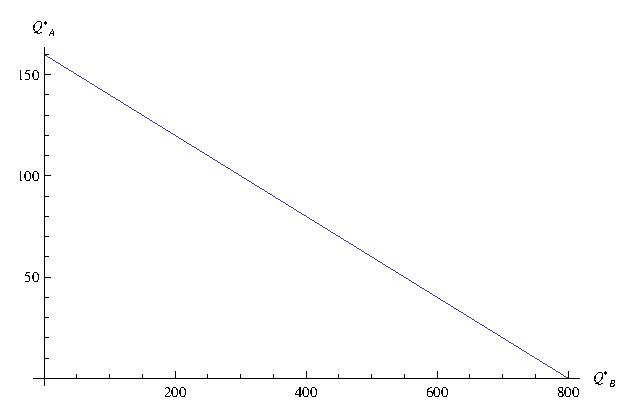
\includegraphics[angle=0, width=0.7\textwidth]{ECON3610A12}
            \end{center}
           (b)
           \begin{center}
                 
\includegraphics[angle=0, width=0.7\textwidth]{ECON3610A13}
           \end{center}
            When the relative price is below $\frac{P_A}{3}$, both countries will specialize in producing bananas.\\ When the relative price is between $\frac{P_A}{3}$ and 5, Home will specialize in apples while the foreign countries will specialize in bananas.\\
            When the relative price is above 5, both countries will produce apples only. \\
        (3)(a)
            \begin{center}
                    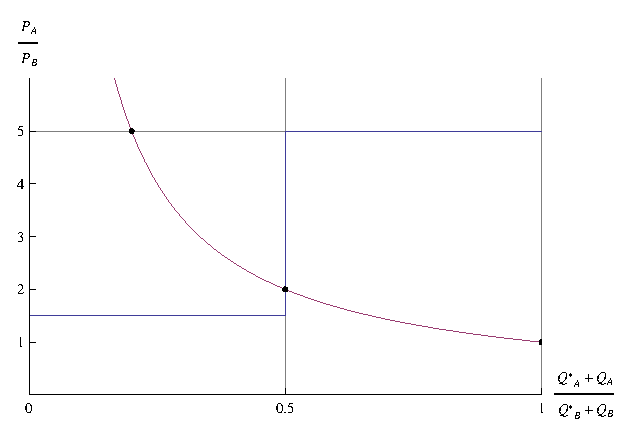
\includegraphics[angle=0, width=0.7\textwidth]{ECON3610A14}\\
            \end{center}
           (b)Equilibrium relative price($P^*$) is 2, the equilibrium relative quantity($Q^*$) is $\frac{1}{2}$.\\
           (c)Home specializes in apples while Foreign only produces bananas.\\
           (d)Domestically, without trade, to produce one more unit of banana, we need to cut down the production of apple by $\frac{2}{3}$ unit. Now, to ``produce'' one more unit of banana, we can use 0.5 unit of apple produced to trade with foreigner. Thus, we lose less to get one more unit of banana. Similarly, foreigners now lose 2 unit of bananas to get one more apple, much less than 5 as before.  \\
        (4) \begin{center}
                    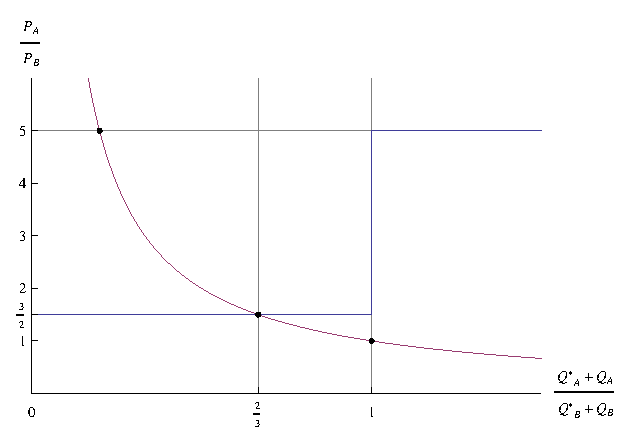
\includegraphics[angle=0, width=0.65\textwidth]{ECON3610A15}
            \end{center}

            Now, there is still gains for foreigners. But whether via trade or not, to get one more banana at Home, the opportunity cost remains $\frac{2}{3}$ unit of apples.\\ So, there is hardly any gains for Home.\\
    \item[III.]{\bf Answer:}\\
        (1)(a)\begin{center}
                    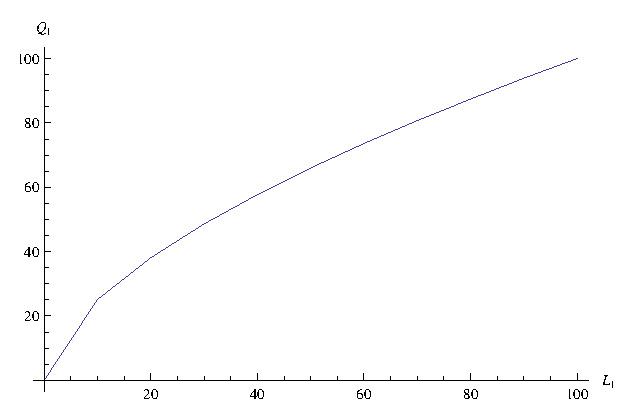
\includegraphics[angle=0, width=0.4\textwidth]{ECON3610A16}
                    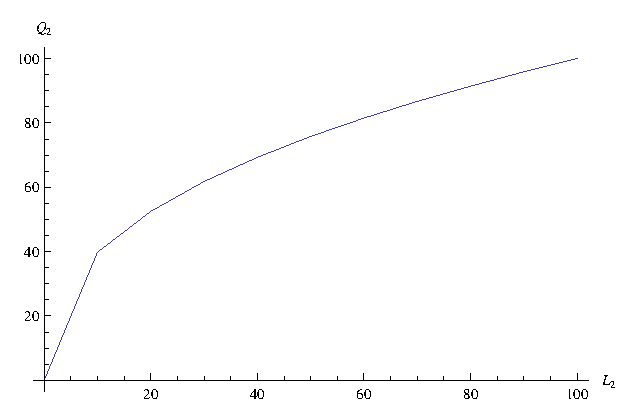
\includegraphics[angle=0, width=0.4\textwidth]{ECON3610A17}
            \end{center}
            $Q_i$ denotes the quantity of Good $i$, and $L_i$ denotes the labor input of Good $i$($i=1,2$).
            \\
           (b)\begin{center}
                    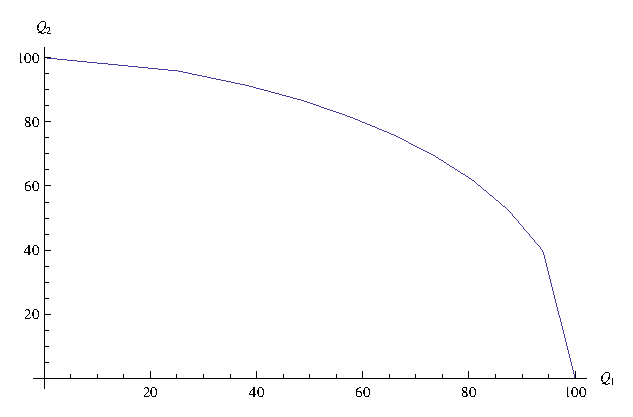
\includegraphics[angle=0, width=0.6\textwidth]{ECON3610A18}
            \end{center}
            The curve is concave to the origin because of the diminishing of MRS. In this particular case, both goods surfer from the diminishing marginal returns. When we produce relatively little Good 1 while relatively much Good 2, to cut down the production of Good 2 by one unit, we will save a lot of labor, which can be used to produce much more good 1. However, When we produce relatively little good 2 while relatively much Good 1, to cut down the production of Good 2 by one unit, we will save nothing much. Thus hardly any Good 1 can be produced by the saving labor, and vice versa.\newpage
        (2)(a)\begin{center}
                    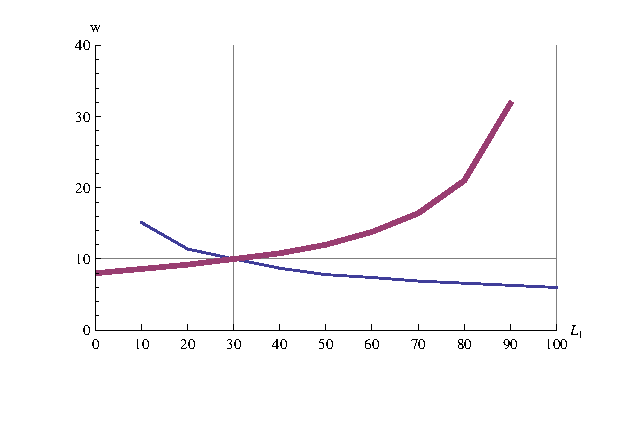
\includegraphics[angle=0, width=0.6\textwidth]{ECON3610A19}
            \end{center}
           (b)$Q_1=48.6$ and $Q_2=86.7$.\\
           \begin{center}
                    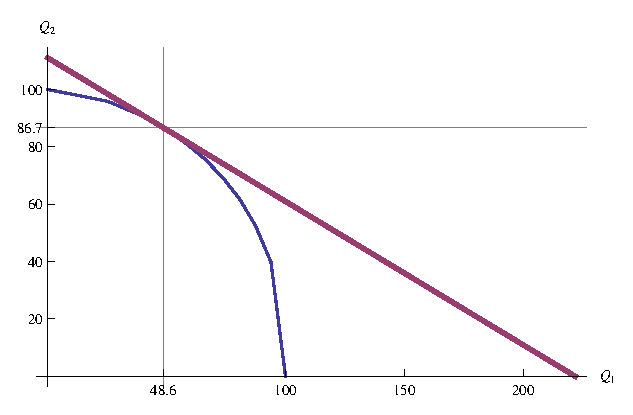
\includegraphics[angle=0, width=0.6\textwidth]{ECON3610A112}
            \end{center}
           (c)\begin{center}
                    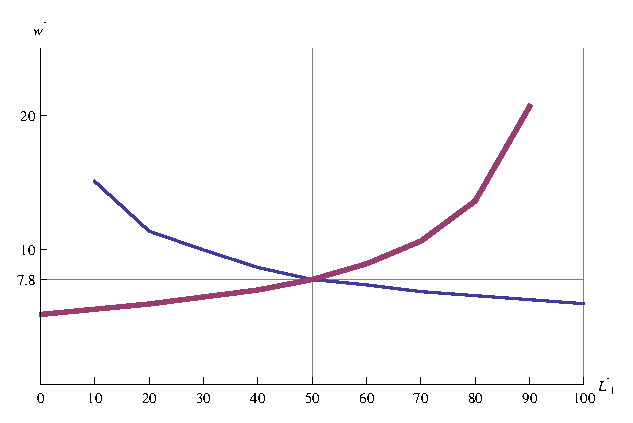
\includegraphics[angle=0, width=0.6\textwidth]{ECON3610A113}
            \end{center}
            Now, $L_1=L_2=50,Q'_1=66$ and $Q'_2=75.8$.\\
            \begin{center}
                    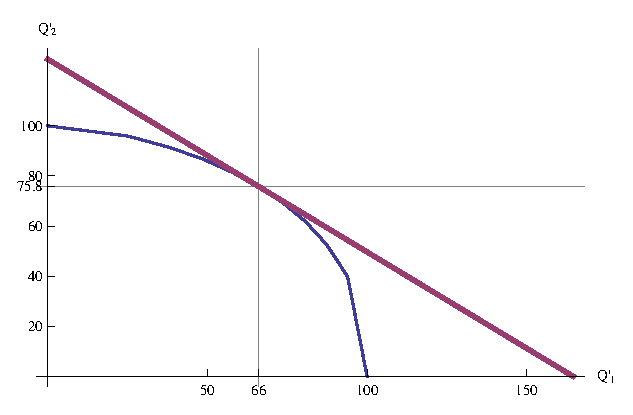
\includegraphics[angle=0, width=0.6\textwidth]{ECON3610A114}
            \end{center}
           (d)
           \begin{align}
           \Pi _c&=P_1\cdot Q_1-w\cdot L_1=1\cdot 48.6-30=18.6\\
           \Pi _{\text{ld}}&=P_2\cdot Q_2-w\cdot L_2=2\cdot 86.7-70=103.4\\
           \Pi '_c&=P'_1\cdot Q'_1-w'\cdot L'_1=1\cdot 66-0.78\cdot 50=27\\
           \Pi '_{\text{ld}}&=P'_2\cdot Q'_2-w'\cdot L'_2=1.3\cdot 75.8-0.78\cdot 50=59.54
            \end{align}
           The income of capital increase by $\frac{27}{18}-1=50\%$, while the income of land decrease by $1-\frac{59.54}{103.4}\doteq 42.4\%$.\\
        (3)(a)
            Because now there is more capital used, more Good 1 will be produced, given any input level of labor.\\
            Let's say: $F\left(K',L_1\right)=F\left(K,L_1\right)\cdot 1.2$\\
            \begin{center}
                    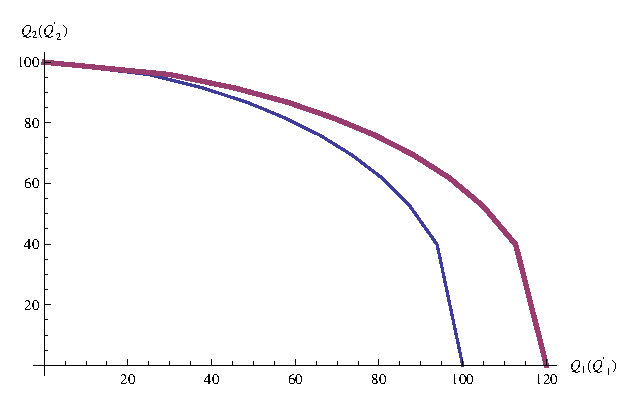
\includegraphics[angle=0, width=0.6\textwidth]{ECON3610A115}
            \end{center}
            Given any Good 2 amount produced, now Home can produce more Good 2.\newpage
           (b)\begin{center}
                    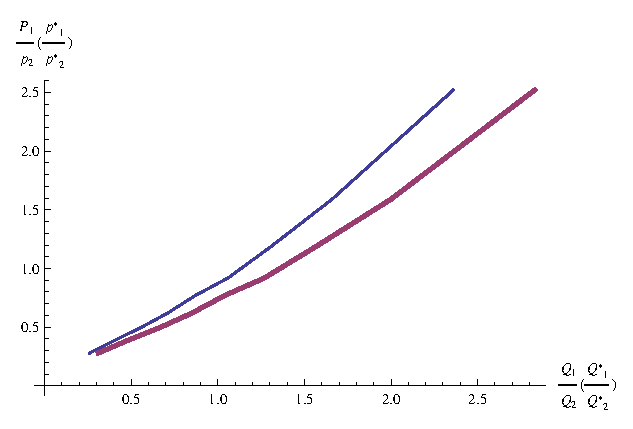
\includegraphics[angle=0, width=0.6\textwidth]{ECON3610A116}
            \end{center}
            where the thicker curve is the relative supply of Home.\\
           (c)Basically, if we assume Home and Foreign have identical demand, (which should not concentrate on only one good) Home will export Good 1 to Foreign and Foreign will export Good 2 to Home.\\
           (d)When opening up to trade, the relative price of Good 1 over Good 2 at Home will fall, thus a downward shift of curve $P_1\cdot \text{MPL}_1$. This eventually lead to the reallocation of workers that some will transfer from sector 1 to sector 2. So, marginal product of capital falls but marginal product of land increase domestically: the landowners are getting better now, but the real and nominal income of capital owners both falls. \\
            Situation changes just the reverse in Foreign: relative price of Good 1 goes up. Foreign owners of capital are better off but their landowners are worse off.\\
           It's hard to evaluate the situation of workers, because the information of their consumption is unavailable. \\


\end{description}
\end{document}
